\documentclass[paper=a4, fontsize=11pt]{scrartcl} % A4 paper and 11pt font size
\usepackage[T1]{fontenc} % Use 8-bit encoding that has 256 glyphs
\usepackage{fourier} % Use the Adobe Utopia font for the document - comment this line to return to the LaTeX default
\usepackage[english]{babel} % English language/hyphenation
\usepackage{fullpage} 
\usepackage{amsmath,amsfonts,amsthm} % Math packages
\usepackage{graphicx}
\usepackage{epstopdf}
\usepackage{eurosym}
\usepackage{hyperref}
\usepackage{lscape}
\usepackage{centernot}
\usepackage{tikz}
\usetikzlibrary{shapes.geometric}
\usepackage{epigraph}
\usepackage{dcolumn}
\usepackage{booktabs}
% \setlength\parindent{0pt} % Removes all indentation from paragraphs - comment this line for an assignment with lots of text
\newcommand*{\mydate}{\today}


%To start each section at a new page
\addtokomafont{section}{\clearpage}


\title{Quantitative Methods of Finance II: Fat Tail Analysis}
\author{Daniel Jorge Deutsch}
\date{\mydate}

\begin{document}
\maketitle
\setcounter{tocdepth}{2}
\tableofcontents


\newcounter{question}
\section{Introduction}
This project aims at estimating climate risks evolution as a a climate economist working for a reinsurance company. Here, I collect data about climate disasters from The Emergency Events Database and estimate the parameters of a Pareto distribution over a rolling window of size 80 years. Later on, the goal becomes to estimate the Value at Risk and the Expected Shortfall considering the whole dataset. 

\section{Dataset}
In order to be able to estimate climate risks evolution, it is necessary to have in hands a dataset about climate events. The dataset chosen for this project consists on records of natural disasters around the globe since 1900. It can be found at the \href{https://public.emdat.be/data}{emdat} website. Once logged in, to obtain the exact same dataset as the one used in this study, all one have to do is select only disasters from a natural cause and, on the location side, lelect all continents. More easily, once you have an account in emdat's platform, the dataset can be downloaded via this \href{https://public.emdat.be/api/files/emdat_public_2022_01_24_query_uid-LeeRPA.xlsx}{url}.

\subsection{Data Content}

As said above, the dataset used in this study contains records of natural disasters since the year 1900. Each row of the dataset consists of 50 columns that provides a wide range of information about the accident going from features like its location and starting date up to damages costs and people affected by it.

\subsection{Data Processing}

Once we have the dataset in hand, it is normal to need to make some changes to it in terms of data types, column names, etc. So, to facilitate the handling of this dataset by the pandas library, all columns have been renamed to snake case format. Also, the pandas library tends to read the dataset and convert its content to the data type "object", which is not the best when we are dealing with numbers. So another important step in data processing is to convert columns with numeric contents to float format. 

\subsection{Data Visualization}

Once the data is in the right format to our analysis, it is very important to first visualize the data in order to understand its necessities and limitations. Notice that the following plots explore the column "Total Damages Adjusted" of the dataset, as it is the one recommended to run our analysis.

\subsubsection{Frequency Over Time}

In the following plot we can see the number of natural disasters per over the last century until nowadays. 

\begin{center}
    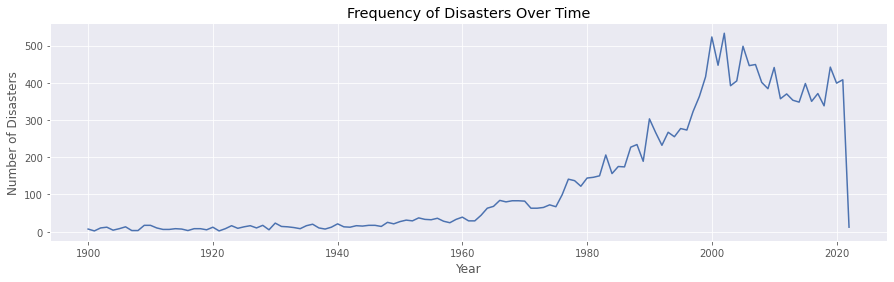
\includegraphics[scale=0.5]{imgs/frequency_of_disasters_over_time.png}
\end{center}

From the plot above, one can clearly see that there is a tendency in increasing the amount of natural disasters over the past century. It is important to say, though, that the lower amount natural disasters in the begining of the 20th century could be due to lack of records of natural disasters at the time (either because of lack of technology or lack of necessity of storing this type of information at the time).

\subsubsection{Total Damages Adjusted Over Time}

On the plot below one can check the adjusted total damages caused by the accidents in each year.

\begin{center}
    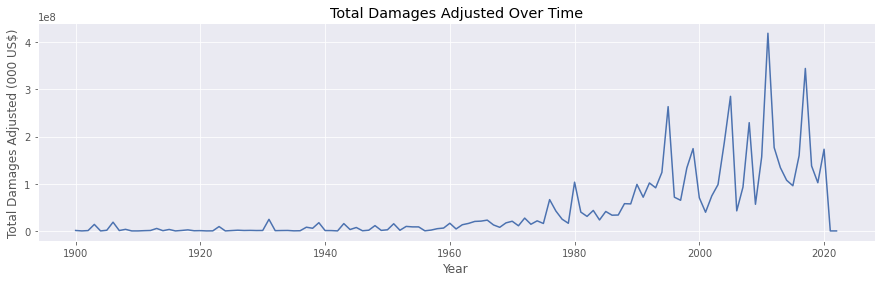
\includegraphics[scale=0.5]{imgs/total_damages_adjusted_over_time.png}
\end{center}

By analyzing the plot above, one can see that the combination of later years disasters tend to have a higher damage when compared to the ones registered in the begining of the past century.

\subsubsection{Histogram of Total Damages Adjusted}

Below, one can check the histogram of total damages Adjusted in log-scale.

\begin{center}
    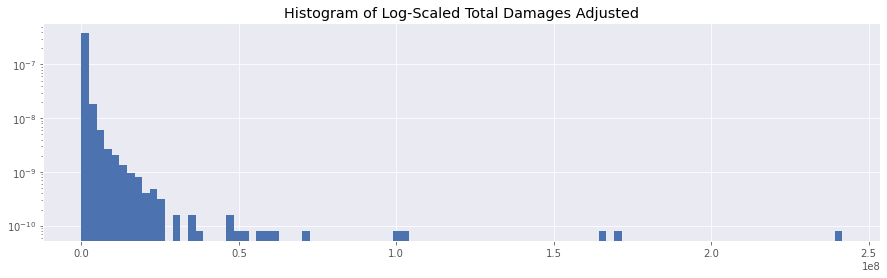
\includegraphics[scale=0.5]{imgs/histogram_log_scaled_total_damages_adjusted.png}
\end{center}

From the plot above its clear to see that there is a higher concentration of disasters that didn't cause a big impact in total damages adjusted.

\section{Rolling Window Estimate}

The goal of this stage of the study is to create a rolling window of size 80 years that rolls through the dataset and for each window, estimate the parameters of one of the Pareto distribution variations seen in class.

\subsection{Stationarity}

Before doing the parameter estimation for one of the Pareto distributions, it is important to verify whether the total damages adjusted time series is stationary or not. To do so, we use the Augmented Dickey Fuller Test.

The Augmented Dickey-Fuller test is a unit root test that checks for stationarity. It considers the following hypotesis:

\begin{align*}
    H_0: & \quad \text{there is a unit root (the series contains a stochastic trend and is non-stationary)} \\
    H_1: & \quad \text{there isn't a unit root (the series doesn't contain a stochastic trend and is stationary)}
\end{align*}

Once the Augmented Dickey-Fuller Test is performed and we have obtained our results, we should consider the following to take our conclusions:

\begin{itemize}
    \item If the p-value is lower than 0.01, than we must reject the null hypotesys (and, consequently, accept the alternativel one).
    \item If the p-value is slightly above 0.01, then the critical values should be used to judge whether to reject the null hypotesis.
\end{itemize}

We, then, implement the augmented Dickey-Fuller Test to the most general regression:

\begin{align*}
    \Delta X_t = b_0 + b_1 t + \rho X_{t-1} + \sum^{p-1}_{j=1} \varphi_j \Delta_{t-j} + \varepsilon_t 
\end{align*}

In this case, the hypotesis can be written as:

\begin{align*}
    H_0: & \quad \rho = 0 \\
    H_1: & \quad \rho < 0
\end{align*}

For the total damages adjusted time series we obtained a T-statistic of -72.027 and a p-value of 0.000. From these results, one can see that the p-value is close to zero, and the T-statistic has a higher absolute value greater than the absolute value of the critical value at 1\% (-4.04). Therefore, we reject the null-hypothesis of non-stationarity.

Once we can consider that the series is stationary, i.e., the total damage adjusted costs  statiscal properties don't change over time, we are able to estimate the time series distribution based on the historical data. 

\subsection{Selection of Pareto Distribution}

As studied in class, there are several variations of the Pareto distribution. This study considers two of them: Pareto Type I and Pareto Type II (or Generalized Pareto).

The first one is bounded from below with $u > 0$ and with tail parameter $\alpha$. Its probability density function $f(x)$ and its cumulative distribution function $F(x)$ are given by:

\begin{align*}
    f(x) & = \frac{\alpha u^\alpha}{x^{\alpha + 1}}
    & \quad
    F(x) & = 1 - \left(\frac{x}{u}\right)^{-\alpha}
\end{align*}

The second one is bounded from below with $u \geq 0$, with scale parameter $\sigma > 0$ and with tail parameter $\alpha \in ]0, +\infty[$. Its probability density function $f(x)$ and its cumulative distribution function $F(x)$ are given by:

\begin{align*}
    f(x) & = \frac{1}{\sigma} \left(1 + \xi \frac{x - \mu}{\sigma}\right)^{-(\frac{1}{\xi + 1})}
    & \quad 
    F(x) & = 1 - \left(1 + \xi \frac{x - \mu}{\sigma}\right)^{-\frac{1}{\xi}}
\end{align*}

In the equations above the $\xi$ variable is the shape parameter, which can be obtained by $\xi = \frac{1}{\alpha}$.

Finally, we fit both distributions to the entire dataset, which yields:

\begin{center}
    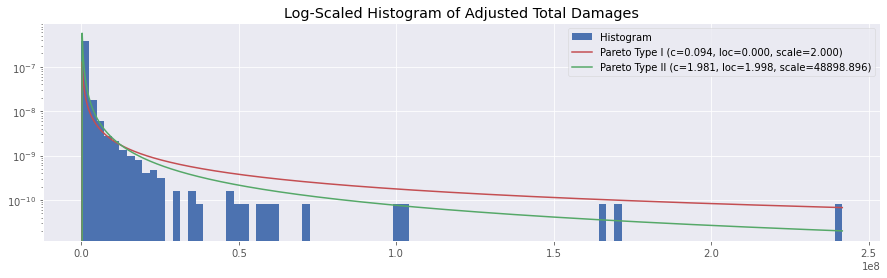
\includegraphics[scale=0.5]{imgs/log_scaled_histogram_adjusted_total_damages.png}
\end{center}

From the plot above, we can observe that the Pareto Type II distribution seems to fit better the data when compared to Pareto Type I. This can be confirmed by the maximized log-likelihood of the distribution models. Calculating this metric on python for both distributions results in:

\begin{center}
    \begin{tabular}{ |c|c|c|c| } 
        \hline
            & Pareto Type I & Pareto Type II \\
        \hline
            Log-Likelihood & -75917.438 & -71152.069 \\
        \hline
    \end{tabular}
\end{center}

As the log-likelihood of the Pareto Type II distribution is greater than the one from Pareto Type I distribution, we can say that this distribution better describes the data.

In spite of observing that the Pareto Type II distribution is a better fit for the data, I decided to pursue the rolling window analysis based on Pareto Type I distribution due to its simplicity of calculations.

\subsection{Pareto Type I Rolling Window Parameter Estimations}

Once the scope of this section is set, all we need to do is estimate the parameters for each window of the rolling window. Since I'm using Pareto Type I distribution to estimate the parameters, it is possible to obtain both $\alpha$ and its upper and lower bound of the confidence interval at 95\% confidence by the following:

\begin{align*}
    \begin{cases}
        \hat{\alpha} & = \left( \frac{1}{N} \sum_{i} (log \ x_i - log \ u) \right)^{-1} \\
        lci & = \left[ \frac{1}{\hat{\alpha}} \left(1 +\frac{2}{N} \right) \right]^{-1} \\
        uci & = \left[ \frac{1}{\hat{\alpha}} \left(1 -\frac{2}{N} \right) \right]^{-1}
    \end{cases}
\end{align*}

Where $N$ is the number of samples in the window and $u$ is the smallest value in the sample.

This yields the following plot:

\begin{center}
    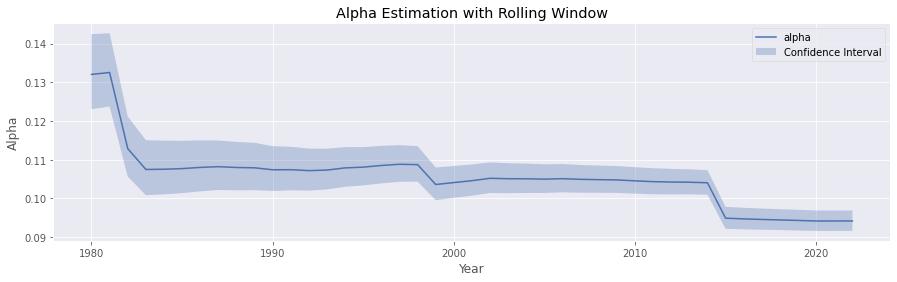
\includegraphics[scale=0.5]{imgs/alpha_estimation_with_rolling_window.png}
\end{center}

From the plot above, one can see that the alphas throughout the rolling window tend to decay as we consider more recent events.


\section{Overall Estimates}
In this section, the idea is to fit the whole total damages adjusted time series into a distribution model and obtain, throught the distribution, its Value at Risk (VaR) and its Expected Shortfall.

For this part of the project, I decided to use the Pareto Type II distribution to fit the data since, as shown before, fits better the data than Pareto Type II.

\subsection{Value at Risk (VaR)}
The value at risk "summarises the worst possible loss of a portfolio at a given confidence level $\alpha \in (0, 1)$ over a given time period $[t, t+1]$. $VaR_\alpha$ is such that the rate of loss of the portfolio won’t exceed that level over that period with a probability inferior or equal to 1 - $\alpha$" - Eric Vansteenberghe. 

For a Pareto Type II distribution, the Value at Risk can be obtained through the following:

\begin{align*}
    \begin{cases}
        u + \sigma \frac{(1 - \alpha)^{-\xi} - 1}{\xi} \qquad & \text{If} \quad \xi \neq 0  \\
        u - \sigma log(1-\alpha) \qquad & \text{If} \quad \xi = 0
    \end{cases}  
\end{align*}

*Note: the $\alpha$ in the above equation is the confidence level, not the Pareto parameter.

Thus, calculating the $VaR_{\alpha=1\%}$ for the given time series we get 225806837.061.

\begin{center}
    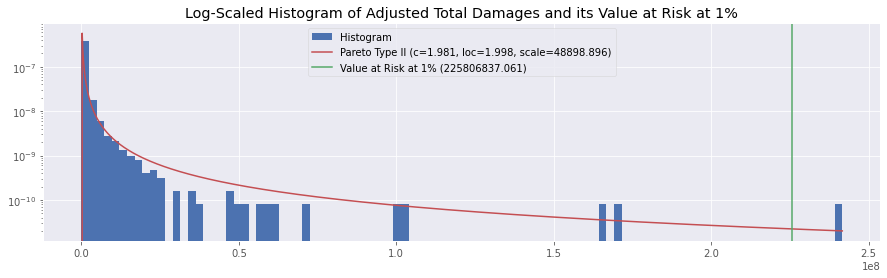
\includegraphics[scale=0.5]{imgs/VaR.png}
\end{center}

\subsection{Expected Shortfall (ES)}

The Expected Shortfall (ES) is the negative of the expected value of the tail beyond the Value at Risk. 

For a Pareto Type II distribution, the Expected Shortfall can be obtained through the following:

\begin{align*}
    \begin{cases}
        \left| u + \sigma \left[\frac{(1-\alpha)^{-\xi}}{1-\xi} + \frac{(1-\alpha)^{-\xi}-1}{\xi}\right] \right| \qquad & \text{If} \quad \xi \neq 0  \\
        u + \sigma [1 - log(1-\alpha)] \qquad & \text{If} \quad \xi = 0
    \end{cases}
\end{align*}

*Note: the $\alpha$ in the above equation is the confidence level, not the Pareto parameter.

Thus, calculating the $ES_{\alpha=1\%}$ for the given time series we get 230313165.371.

\begin{center}
    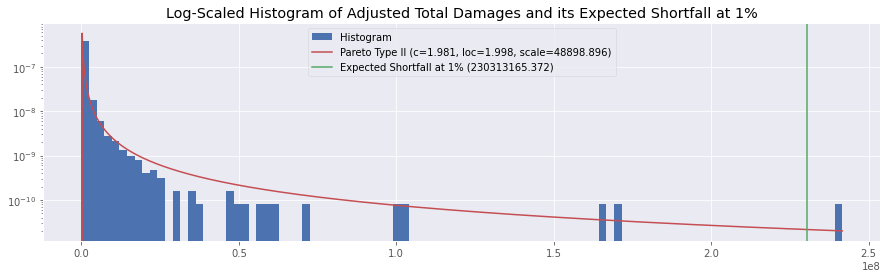
\includegraphics[scale=0.5]{imgs/ES.png}
\end{center}

\section{Conclusion}
Given the results obtained in section 3.3 we can conclude that as, the values of the alphas in the Pareto Type I distribution tends to decrease over the windows that considers more recent years, the tail of the distribution tends to be "higher" and, therefore, natural accidents tend to have a higher total damage adjusted in recent years. Apart from that, section 4.1 shows that the worst loss that one can expect during a one year period with a confidence level at 1\% is 225806837.061. Finally, section 4.2 shows that the total damage adjusted that one expect to be, on average, when an event exceeds the Value at Risk with a 1\% confidence level is 230313165.371.


\newpage
\begin{thebibliography}{9}
    \bibitem A Quantitative methods in finance, Eric Vansteenberghe, January 29, 2022.
\end{thebibliography}

\end{document}


